\chapter{Construction of Occurrence Graph Grammars with NACs}\label{ch:tests}

%A test case is a collection of (1) input values necessary to complete some execution of the system under testing, (2) the results that must be produced after executing the test (assuming the system satisfies the intended behaviour) and (3) any inputs necessary to setup the system into the appropriate state to receive the test values~\cite{Ammann2008}.
%Test oracles are specifications describing properties about the validity of tests cases, i.e. if the test must fail or pass. These properties may include relationships between the input given and the expected output, data validity properties, format of possible execution paths, etc. No matter the oracle format, it must be able to determine the validity of tests in a finite and reasonable amount of time~\cite{Weyuker1982}.

%In the following, we show how to use \newadd{deterministic} occurrence graph grammars to generate test cases and oracles from (simply-typed) graph grammars modelling systems. In theory, this approach can be used to generate tests for any graph grammar\footnote{\newadd{Assuming the grammar follows the DPO approach with incremental NACs}}, since it is based only on the properties of the formalism. However, we focused on graph grammars that were generated from use cases by using the methodology presented in \cite{Junior2015}, \cite{BezerraWEIT2016} and \cite{Cota2017}.

%This methodology is a systematic, computer-aided way to extract graph grammars from use cases or other text-based requirement documents. At the same time, it helps finding problems such as ambiguities, inconsistencies and omissions in the documents. Thus, providing a better specification and also an improved model. By generating tests from these grammars we are indirectly generating tests for the underlying use cases. The test generation, to be described in next sections, was implemented in Verigraph as an extension of the previously discussed calculation of occurrence graph grammars.

%We focused our approach on testing the integration of different functionalities (or requirements) of a system. By \emph{functionality}, we informally mean an aim the system is supposed to accomplish, which has value to a user or any other stakeholder. By \emph{integration} we mean the emergent behaviour of executing several functionalities, possibly multiple times.

% In the graph grammar model of a system, a functionality can be represented either as a single rule or as a collection of rules. In either case, those rules must be executed to achieve the functionality goals. Therefore, the main idea of our approach is that, given a collection of functionalities, we find out whether it is possible to find a sequence in which all these functionalities can be performed, then we characterize the assumptions that must be satisfied for them to be performed and/or the restrictions that may prevent their execution. Given a collection of functionalities modelled as graph rules, we are interested in generating:

\iffalse
\begin{enumerate}
\item the minimal input data necessary for these functionalities to execute, as well as the output data of a successful execution;
\item at least one path in which all functionalities can be applied (if possible);
\item a set of constraints two characterize any test into those which should pass and those which should fail;

\hide{
\item a set of constraints which can tell which intermediate states of the system are valid and those that are not.}
\end{enumerate}

Notice that the two first items correspond to test cases while the last one correspond to test oracles.
\fi
%First, we present a brief overview of the methodology for extracting graph grammars from use cases, after what we present the process of generating the tests cases from the extracted grammars.

In this chapter, we present the process of constructing Occurrence Graph Grammars with NACs (OGGs) in a systematic manner and how this process was implemented in Verigraph. We make use of some example grammars in order to illustrate the explanation. We also applied this process in more complex graph grammars: One of the grammars models the system of a restaurant, with functionalities such as login of employees, reservation and cancellation of tables,
accommodation of clients, serving tables, among others. Another models the system of an e-Store, with functionalities such as browse and search catalogue, registration of clients, login, maintain shopping cart, effectuate purchase, etc. The grammars, their textual specifications (use cases), together with their generated OGGs can be found at the Verites repository for case studies\footnote{https://github.com/Verites/case-studies}.



%that modelling the system of a restaurant and , built from the set of use cases presented in Appendix~\ref{app:use-cases} by applying the systematic methodology proposed by~\cite{Junior2015}. These use cases model basic functionalities of the proposed restaurant system such as login of employees, reservation and cancellation of tables, accommodation of clients, serving tables, among others. The complete extracted grammar, together with its generated OGGs can be found at the Verites repository for case studies\footnote{https://github.com/Verites/case-studies}.

Our first example is the \emph{Mail Server Graph Grammar} presented on chapter~\ref{ch:gts}, which will be reintroduced. Then we proceed to the explanation of the necessary steps to build an Occurrence Graph Grammar according to the definitions presented on chapter~\ref{ch:process}. Our second example is a \emph{Traffic-Light Graph Grammar}, which will be introduced later on this chapter and also used to explain the process of constructing an OGG. The implementation of this process in Verigraph is also part of this thesis contribution, as Verigraph is the first tool in the field to implement the construction of Occurrence Graph Grammars, even when considering OGGs without NACs. As a possible practical application of this, at the end of the chapter, we provide some insight about how OGGs can be used to generate test cases for the system they model.
%Given the graph grammar model of a system, we want to generate test cases and oracles for collections of its underlying functionalities. These collections could represent something as ``atomic'' as a successful or failing login attempt or something as complex as the entire workflow of attending clients, which would require attendants and waiters to log in into the system, tables to be occupied, orders to be prepared, among possibly several other steps.

%The reason why we focused on collections of functionalities is to test the emergent behaviour of a system, which usually is not observable if we consider each functionality in isolation. By grouping together several (usually, but not necessarily different) functionalities, we may realize how they interact with each other and which are the overall effects of this integration.

%\begin{definition}[Functionality Collection] Given a graph grammar \graphGrammar{} that models a system, a \emph{functionality collection} $F$ is a collection of its grammar rules. The term collection here is used instead of set to imply that the same rule $r \in P$ can appear more than once in $F$. In this context, it means the functionality modelled by $r$ is intended to be executed more than once.
%\end{definition}

%\section{Running Example}

\begin{example} %The rules we chose for this example represent one way in which the entire process of serving a client can be accomplished. In this particular case, we chose the rules representing the successful paths of the use cases \emph{reserve table}, \emph{accommodate client}, \emph{serve table} and \emph{close table}, which are depicted on figure~\ref{fig:tests:grammar}.
  The grammar used here illustrates a mail server scenario for a simple e-mail application composed by four rules, which are described in the following and depicted in Figure~\ref{fig:tests:grammar}.
  In order to better present the ideas of this chapter in terms of its implementation, we use the rules in the format provided by AGG~\cite{Taentzer2000}, which is also the format used as input and output by Verigraph.
  This format depicts the LHS and RHS graphs of rules, but does not explicitly show the interface graph, which can be inferred by identification numbers correlating items of LHS and RHS.

\begin{enumerate}[label=(\alph*),start=1]
  \item \emph{Send message:} a client writes a message which they send to a server, however there is a NAC forbidding the message of being sent if it has a piece of data attached to it.
  \item \emph{Get data:} a piece of data is obtained from a server and attached to a message.
  \item \emph{Receive message:} a server sends a message with attached data to a client.
  \item \emph{Delete message:} a client obtains a piece of data from a received message and this message is destroyed.
\end{enumerate}
\end{example}
%
%\begin{description}
%  \item[Reserve table:] A receptionist of the restaurant tags a table as reserved for a specific client at a given date and time. Therefore, this table must not be allocated for another client, either by accommodation or reservation, at the same time.
%  \item[Accomodate client without reservation:] A receptionist leads a client to a free table, then notifies the system that this table is waiting for service.
%  \item[Serve table:] A waiter goes to an occupied table to take an order, adding or removing items to/from the order, then closing it and sending it to the kitchen to be prepared.
%  \item[Close table:] A waiter goes to a table that has been serviced, closes the corresponding bill and collects the payment from its client.
%\end{description}

\begin{figure}[!ht]
  \centering
  \begin{subfigure}[t]{.5\textwidth}
    \centerline{\fbox{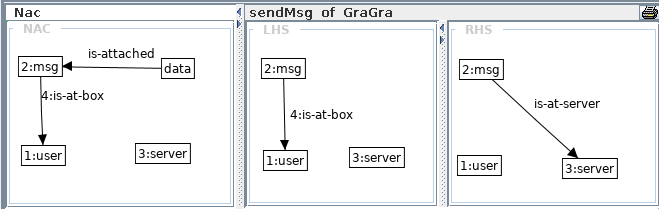
\includegraphics[scale=0.5]{grammar/server/sendMsg}}}
    \caption{Rule \emph{send message}}
  \end{subfigure}
  \begin{subfigure}[t]{.5\textwidth}
    \centerline{\fbox{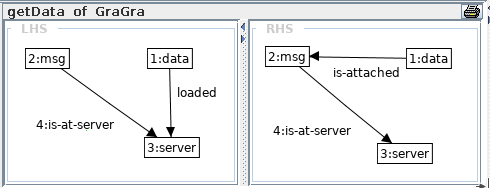
\includegraphics[scale=0.5]{grammar/server/getData}}}
    \caption{Rule \emph{get data}}
  \end{subfigure}
  \begin{subfigure}[t]{.5\textwidth}
    \centerline{\fbox{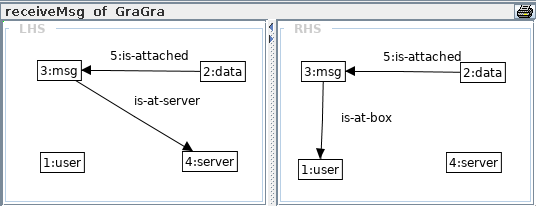
\includegraphics[scale=0.5]{grammar/server/receiveMsg}}}
    \caption{Rule \emph{receive message}}
  \end{subfigure}
  \begin{subfigure}[t]{.5\textwidth}
    \centerline{\fbox{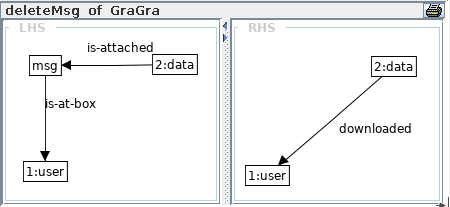
\includegraphics[scale=0.5]{grammar/server/deleteMsg}}}
    \caption{Rule \emph{delete message}}
  \end{subfigure}
  \caption{Rules for a mail server application}\label{fig:tests:grammar}
\end{figure}

\section{Selecting a Computation of GG}

  In this work we defined only deterministic Occurrence Graph Grammars with NACs, and therefore, in contrast to~\cite{Ribeiro1996}, where the semantics of a Graph Grammar is represented by only one (non-deterministic) Occurrence Graph Grammar, here we need a set of Occurrence Graph Grammars to represent the behaviour of a Graph Grammar.
  Nevertheless, this set is usually much smaller than the set of all derivations of a Graph Grammar since each OGG represents a (shift-)equivalent set of derivations, that is, a set of derivations that are equivalent with respect to switching the order of independent steps. 
  In the following we will describe how to construct one OGG, the complete behaviour of a GG would be described by the (possibly infinite) set of OGGs that can be constructed with the rules of the underlying GG. Note that, even in the case of~\cite{Ribeiro1996}, where the semantics was described by only one OGG, this structure may be  infinite in the case the system has the possibility of a non-terminating computation.

  Thus, in order to construct an Occurrence Graph Grammar $OGG$ for a graph grammar \graphGrammar{}, we need (1) a collection\footnote{ We use the term collection instead of set because, in this case, a rule can appear more than once since each rule in $F$ represents the application of a rule in $P$.} of rules $F$ based on $P$, which represent the rules that are applied in the computation depicted by the OGG, and (2) a way of specifying how the rules in $F$ interact among themselves. 
  The latter is needed to define which elements are common throughout the rules. To this purpose, we use an \emph{input-output relation}, depicting connections between the rules in $F$.
  The objects in this relation identify which elements must be the same between pairs of rules.
  This construction is similar to the construction of concurrent rules in AGG.
  The difference is that instead of building a rule, the result of our construction is an OGG, i.e., represents a computation.

\begin{definition}[Input-Output Relation] Given a collection $F$ of rules, an \emph{input-output relation} $IO$ over $F$ is a set of typed-graph morphism spans of the form \mbox{$R_x \leftarrow IO_i \rightarrow L_y$} each of which connects two distinct rules $x,y \in F$.
\end{definition}

The $IO_i$ object of each span works similarly to the gluing graph $K$ of a rule, but instead of identifying elements that are the same in both left and right sides of a single rule, it identifies elements that are necessarily the same between the right and left sides of two different rules. An input-output relation for a collection of rules will have an appearance similar (but not necessarily equal) to the following diagram, where there are several $IO$ objects connecting the right-hand side of a rule with the left-hand side of another one.

\diagram{
  & & & & IO_6\ar@{-->}[dddrrrr]\ar@{-->}[dddllll] & & & &\\
  & IO_3\ar@{-->}[ddl]\ar@{-->}[ddrrrr] & & & & & & IO_4\ar@{-->}[ddr]\ar@{-->}[ddllll] &\\
  & & IO_1\ar@{-->}[d]\ar@{-->}[dr] & & IO_5\ar@{-->}[drr]\ar@{-->}[dll] & & IO_2\ar@{-->}[d]\ar@{-->}[dl] & &\\
  L_1 & K_1\ar[l]\ar[r] & R_1 & L_2 & K_2\ar[l]\ar[r] & R_2 & L_3 & K_3\ar[l]\ar[r] & R_3\\
  }


\begin{remark}We could have have also included in the $IO$ relation a type of span that also connects only the left (resp. right) sides of rules together, however we would accomplish very little with this kind of span. Given that we are looking for Occurrence Graph Grammars, where the exact same element can not be deleted or created by two different rules, this particular kind of span would serve only to identify elements that are preserved by both rules, otherwise they would introduce inconsistencies, therefore preventing the creation of OGGs.
\end{remark}

\begin{example}[Input-Output Relations]\label{ex:inout} Figure~\ref{fig:tests:inout} shows one possible $IO$ relation for our running example. Notice that the elements which should be the same in both rules have the same prefix number in their identification. The first $IO$ object connects the rules \emph{send message} and \emph{get data}.  In this case, we want the server, the message and the connection between them to be the same in both rules. %For example, the table involved in both action is the same table, as a client there is accommodated must also be served. The employees, on the other hand, are not, as the employee who receives the client in the restaurant (the receptionist) is not the same who serves the client (the waiter).

As a side note, the reader may notice that it is not mandatory to create an $IO$ span \mbox{$\left(R_x \leftarrow IO_i \rightarrow L_y\right)$} for \textbf{every} pair of rules. For example, consider that we want to analyse a scenario where the \emph{server} node is unique. Given rules \emph{get data} and \emph{receive message}, we have the options of building the span that identifies the server node as
  $R_{sendMsg} \leftarrow IO_n \rightarrow L_{receiveMsg}$ or $R_{receiveMsg} \leftarrow IO_m \rightarrow L_{sendMsg}$, or even combining the two of them. Any option would result in the same final effect: both rules use the same \emph{server}.
  \begin{figure}[!ht]
  \centering
  \fbox{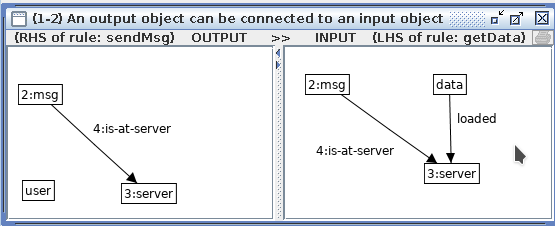
\includegraphics[scale=0.5]{grammar/server/io-object}}
  \fbox{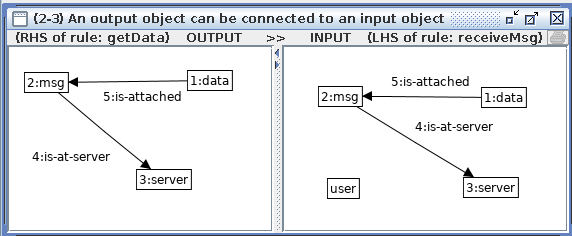
\includegraphics[scale=0.5]{grammar/server/io-object2}}
  \fbox{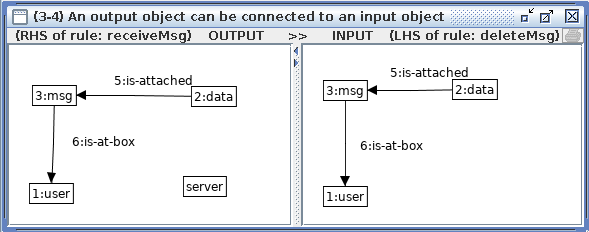
\includegraphics[scale=0.5]{grammar/server/io-object3}}
  \caption{A basic Input-Output relation building}\label{fig:tests:inout}
\end{figure}
\end{example}

Currently, the generation of the \textit{input-output relation} is a manual step in our strategy, therefore the analyst needs to decide how to better implement his/her own $IO$ relation. This did not shown to be a problem, as in our analysis we usually wanted to restrict the number of possible combinations to more realistic cases. However, its fully automation was scheduled as future work.


\section{Constructing the OGG}

  Having $GG$, the graph grammar model of the system; $F$, a collection of rules; and $IO$, an \emph{input-output relation}, we proceed to the construction of an occurrence graph grammar for $GG$ accomplished by means of an amalgamation of $F$ over its input-output relation $IO$.
  This amalgamation is later used in the construction of a doubly-typed graph grammar, which we then check to verify whether it satisfies the conditions to be an occurrence grammar. The construction steps are specified in
  Definition~\ref{def:ogg-construction}, which is an adaptation of the construction of an occurrence graph grammar without NACs from~\cite{Corradini1996}.

\begin{definition}[Deterministic Occurrence Graph Grammar Construction]\label{def:ogg-construction} Given a grammar \graphGrammar{}, $F$ a collection of rules from $P$, and $IO$ and input-output relation over the rules in $F$:

\begin{enumerate}
  \item\label{enum:construction-colimit} calculate the amalgamation (colimit) $Occ$ of the rules in $F$ with respect to $IO$ as presented in the following diagram, where all squares commute.

\diagram{
  & & & & IO_6\ar[dddrrrr]\ar[dddllll] & & & & \\
    & IO_3\ar[ddl]\ar[ddrrrr] & & & & & & IO_4\ar[ddr]\ar[ddllll] &\\
    & & IO_1\ar[d]\ar[dr] & & IO_5\ar[drr]\ar[dll] & & I O_2\ar[d]\ar[dl] & &\\
    L_1\ar[dddrrrr] & K_1\ar[l]\ar[r] & R_1\ar[dddrr] & L_2\ar[dddr] & K_2\ar[l]\ar[r] & R_2\ar[dddl] & L_3\ar[dddll] & K_3\ar[l]\ar[r] & R_3\ar[dddllll]\\
    & & & & & & & &\\
    & & & & & & & &\\
    & & & & Occ & & & &
}\hfill\break

\hide{
\diagram{
  & & & & IO_6\ar[dddrrrr]\ar[dddllll] & & & & &\ldots\\
    & IO_3\ar[ddl]\ar[ddrrrr] & & & & & & IO_4\ar[ddr]\ar[ddllll] & & \ldots\\
    & & IO_1\ar[d]\ar[dr] & & IO_5\ar[drr]\ar[dll] & & IO_2\ar[d]\ar[dl] & & &\ldots\\
    L_1\ar[dddrrrr] & K_1\ar[l]\ar[r] & R_1\ar[dddrr] & L_2\ar[dddr] & K_2\ar[l]\ar[r] & R_2\ar[dddl] & L_3\ar[dddll] & K_3\ar[l]\ar[r] & R_3\ar[dddllll] & \ldots\ar[dddlllll]\\
    & & & & & & & & &\\
    & & & & & & & & &\\
    & & & & Occ & & & & &
}\hfill\break}

\item \emph{retype} the rules in $F$ over $Occ$: use each morphism found from each $L_i, K_i, R_i$ to $Occ$ as their respective new typing morphism. This step generates a set $F'$ of doubly-typed graph rules, given that $Occ$ is a $TG$-typed graph itself.

\item calculate the causal relation $\leq_{c}$ of the doubly-typed graph rules in $F'$ and verify whether it is a partial order.

\item\label{enum:construction-graphs} generate the initial and final graphs $I$ and $J$ by respectively deleting from $Occ$ all elements ever created and deleted by the rules in $F'$.

\item\label{enum:construction-occurrence} calculate and categorize the produce-forbid conflicts and delete-forbid dependencies according to definitions~\ref{def:delete-forbid-strong} and~\ref{def:produce-forbid-strong}.

\begin{enumerate}
\item\label{enum:construction-analysis} use the concrete conflicts and dependencies to extend the causal relation in order to obtain the occurrence relation $\leq_o$.

\item\label{enum:construction-restriction} use the abstract conflicts and dependencies to generate the set $R$ of restrictions over the ordering of rules applicability.
\end{enumerate}

\item\label{enum:construction-ordering} find one or more total orderings of rules in $F'$ which respects both the occurrence relation and the occurrence restrictions.
\end{enumerate}

%  The (Deterministic) Occurrence Graph Grammar representing execution of the functionality $i$ is given by $OGG_i = (Occ_i, I_i,F_i)$, iff $OGG_i$ respects the conditions imposed by Definition~\ref{def:ogg} 
\end{definition}

If all the steps in such a construction can be successfully executed, specially steps~\ref{enum:construction-graphs} and~\ref{enum:construction-ordering}, we have that $OGG = (Occ, I, F')$ is not only a doubly-typed graph grammar, but also a deterministic occurrence graph grammar. %This means it is possible to successfully apply all the rules in the original collection $F$. %Our approach creates test cases and oracles from $OGG$ whether it is in fact an occurrence graph grammar or not. In the first case, we have tests for success and failure execution paths, whereas in the second we have tests only for the failure ones. Notwithstanding, we regard the failure tests as important because they pinpoint uses of the underlying system where the system itself is supposed to fail, therefore they can not or should not be performed. In the following, we dive into details of each construction step.

The first step of the construction, the amalgamation of rules in $F$ w.r.t. $IO$, is responsible to ``glue'' the graphs of all rules in one typed graph $Occ$, while identifying the items that are meant to be the same throughout the grammar execution. This can be regarded as a mapping which turns generic elements such as \textit{a user} into concrete elements such as the user named \textit{Bob}. It also discriminates these elements, for instance: the user \textit{Bob} is different from the user
\textit{Alice}. Therefore, at the end of this step, $Occ$ contains all concrete elements ever to be created, preserved or deleted by any of the rules in collection $F$. Figure~\ref{fig:tests:amalgamation} shows the amalgamation of an $F$ containing one copy of each rule in our example grammar w.r.t. the IO relation depicted on Figure~\ref{fig:tests:inout}.

\begin{figure}[!ht]
  \centering
  \fbox{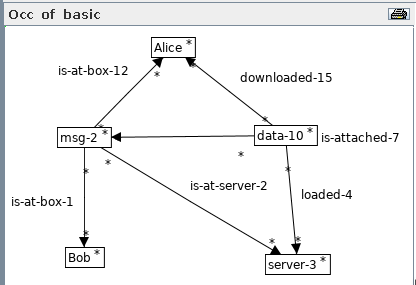
\includegraphics[scale=0.5]{grammar/server/amalgamation}}
  \caption{Amalgamation (colimit) of rules according to the basic IO relation.}\label{fig:tests:amalgamation}
\end{figure}

The retyping step is responsible for generating actions: ``new'' graph rules which, rather than being generic descriptions of system transformations, represent concrete executions of the original rules over a given context. Therefore, a rule which describes the process where a user receives from the server a message sent by another\footnote{Notice that the original graph grammar does not specify that the sender must be different from the receiver, therefore we would be able to choose a
computation where they are the same user.} user becomes a concrete action where \textit{Alice} receives \textit{the message} sent by \textit{Bob}.
%The set $F'$ of doubly-typed graph rules from the colimit calculated in the previous step.
For each graph rule $\mbox{$p_i^{TG} = \left(L_i^{TG} \leftarrow K_i^{TG} \rightarrow R_i^{TG}\right)$} \in F$, we generate a new action \mbox{$q_i^{Occ} = \left(L_i^{Occ} \leftarrow K_i^{Occ} \rightarrow R_i^{Occ}\right) \in F'$}, where the typing morphisms are those from the original rules in $F$ to the colimit graph $Occ$. Since $Occ$ is the type graph of the new rules and, at the same time, a typed graph over $TG$, the actions are now doubly-typed rules over $Occ^{TG^T}$.
Figure~\ref{fig:tests:actions} shows the actions generated for our running example\footnote{ Since we use AGG as our form of output visualization and it was not intended to provide support for doubly-typed graph grammars, the NACs of our actions can not be properly seen, however they are maintained and used in Verigraph internal format.}.

\begin{figure}[!ht]
  \centering
  \begin{subfigure}[t]{.5\textwidth}
    \centerline{\fbox{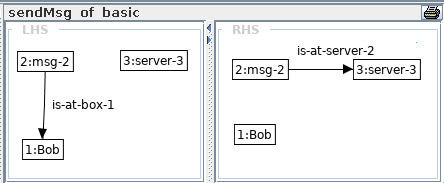
\includegraphics[scale=0.5]{grammar/server/amalgamation/sendMsg}}}
    \caption{Rule \emph{send message}}
  \end{subfigure}
  \begin{subfigure}[t]{.5\textwidth}
    \centerline{\fbox{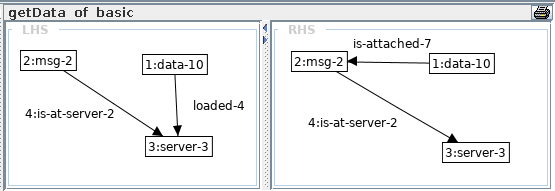
\includegraphics[scale=0.5]{grammar/server/amalgamation/getData}}}
    \caption{Rule \emph{get data}}
  \end{subfigure}
  \begin{subfigure}[t]{.5\textwidth}
    \centerline{\fbox{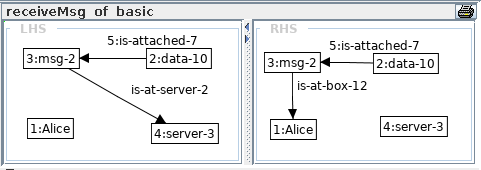
\includegraphics[scale=0.5]{grammar/server/amalgamation/receiveMsg}}}
    \caption{Rule \emph{receive message}}
  \end{subfigure}
  \begin{subfigure}[t]{.5\textwidth}
    \centerline{\fbox{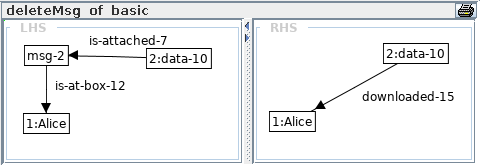
\includegraphics[scale=0.5]{grammar/server/amalgamation/deleteMsg}}}
    \caption{Rule \emph{delete message}}
  \end{subfigure}
  \caption{The set of actions generated w.r.t. our basic $IO$ relation}\label{fig:tests:actions}
\end{figure}

Once the set $F'$ of actions was created, we proceed to calculating the causal relation, as described in Definition~\ref{def:causal-relation}. This relation is the very first indicative of whether it is possible to construct an occurrence graph grammar for the given collection of rules. Remember that this relation must be a partial order, otherwise the totality of rules in $F$ are not executable. Specifically, the causal relation gives us hints over the order in which the actions must be performed to accomplish the functionality aims, for example: \textit{Bob} must sent \textit{the message} to \textit{the server} before it reaches \textit{Alice}. The occurrence relation of our example is [getData < deleteMsg, getData < receiveMsg, receiveMsg < deleteMsg, sendMsg < deleteMsg, sendMsg < getData, sendMsg < receiveMsg]. It is also easy to see that this relation is a partial order. In fact, there is only one possible total order derived from it: $[sendMsg < getData < receiveMsg < deleteMsg]$.

The next step consists of using the causal relation and the graph $Occ$ in order to generate the initial and final graphs of our target grammar. These graphs correspond to the necessary input and expected output of performing $F$ in a minimal context. In order to create the graphs, we delete from $Occ$ the elements that are created (resp. deleted) by the rules in $F'$ according to the causal relation. For example: \textit{Alice} is a person who can never be created by any action of our system, no matter how advanced, as a consequence she must be present in any initial states of the actions performed with her. \textit{The message} sent by \textit{Bob} was never created by any action either, so it must be present in the initial graph. However, it is deleted by the action \emph{deleteMsg}, so it must not appear in the final graph.

\begin{figure}[!ht]
  \centering
  \begin{subfigure}[t]{.5\textwidth}
    \centerline{\fbox{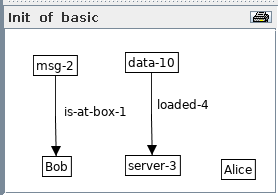
\includegraphics[scale=0.6]{grammar/server/initial}}}
    \caption{Initial graph}
  \end{subfigure}%
  \begin{subfigure}[t]{.5\textwidth}
    \centerline{\fbox{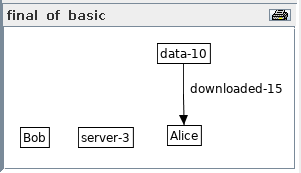
\includegraphics[scale=0.6]{grammar/server/final}}}
    \caption{Final graph}
  \end{subfigure}
  \caption{Instance graphs}\label{fig:tests:graphs}
\end{figure}

In general, after simply deleting those elements from $Occ$, the result may be that either \emph{Initial} or \emph{Final} graphs are not valid, in the case that any source or target node of an edge is deleted, but not the edge itself. This means that the execution of $F$ would need to begin on or lead to an inconsistent state, therefore no sequencing of actions in $F$ could be performed in a real execution. However, if they are indeed valid graphs, as they are in our example, we have just found the initial and final (minimal) states of the system regarding the execution of all rules in $F$.

Notice that, if the steps listed so far (\ref{enum:construction-colimit} to~\ref{enum:construction-graphs}) were able to be successfully performed, we have a grammar \mbox{$OGG = \left(Occ, I, F'\right)$} that is not only doubly-typed, but also strongly safe in the sense of Definition~\ref{def:strongly-safe-grammar}. Therefore it is a candidate to be an occurrence graph grammar.

In step~\ref{enum:construction-occurrence}, we proceed towards creating the occurrence relation and occurrence relation restrictions. 
  In~\ref{enum:construction-analysis}, we calculate all produce-forbid conflicts and delete-forbid dependencies between the rules in $F'$ by using the categorial algorithms presented in Definitions~\ref{def:delete-forbid-strong} and~\ref{def:produce-forbid-strong}. 
  Initially, we do not know whether these conflicts and dependencies will be exercised during the execution of the underlying grammar. 

  In our example, we find one conflict and one dependency induced by NACs. The first is a produce-forbid between \emph{getData} and \emph{sendMsg} regarding the creation of the attachment between the piece of data and the message in \emph{getData}, which is forbidden by the NAC of \emph{sendMsg}.
  The second, a delete-forbid between \emph{deleteMsg} and \emph{sendMsg}, regarding the deletion of that same attachment.
  Given the information collected so far we can deduce whether any of these
conditions exists in the local context.
  Hence, we use the information acquired in previous steps to classify those conflicts and dependencies as concrete, abstract or non-existent as specified in
Definitions~\ref{def:delete-forbid-strong} and~\ref{def:produce-forbid-strong}. 

In this particular case we already know, by looking at the causal relation, that \emph{sendMsg} must be executed before \emph{getData}, therefore the later action can never trigger the NAC of an action that occurs before it, and this conflict is non-existent. Similarly, for the delete-forbid, as we know that the condition that triggers the NAC of \emph{sendMsg} does not exist prior to any possible of its executions, it is not necessary for \emph{deleteMsg} to remove the element triggering the NAC, therefore this dependency is also non-existent.

The occurrence relation $\leq_o$ is then calculated from the causal relation together with the concrete conflicts and dependencies. In step~\ref{enum:construction-restriction} we create the set $R_i$ of restrictions as the union of all abstract conflicts and dependencies calculated before. In our example, since no concrete conflicts or dependencies were found, the occurrence relation remains equal to the causal relation. As for the set of restrictions, since no abstract conflicts or dependencies
were found, it remains empty.

Finally, we have the strongly safe grammar $OGG$ together with its corresponding occurrence relation $\leq_o$ and a set of restrictions $R$. As it was shown, if $\leq_o$ is a partial order and it is possible to find a total ordering of it that respects all restrictions in $R$, it follows that $OGG$ is an occurrence graph grammar according to Definition~\ref{def:ogg}.
\linebreak

  In our previous example, no situation with abstract conflicts or dependencies was found.
  This grammar and the particular execution chosen have a causal relation which forces a sequencing of actions that avoids the existence of abstract conflicts/dependencies.
  In our case studies, this situation has shown to be very common in graph grammars extracted from use cases, where there are clear steps that must be followed in a specific order to accomplish the completion of a functionality.
  Nonetheless, in graph grammars that model systems with higher parallelism or concurrency, situations with abstract conflicts/dependencies have shown to arise more often. We now introduce another graph grammar example with more independent rules to illustrate the construction of an occurrence graph grammar with NACs which has a non-empty set of restrictions.

\begin{example} This graph grammar models a common traffic situation, where a pedestrian crosses or not a street according to the state of a traffic light. The grammar is depicted in Figure~\ref{fig:tests:grammar-traffic} while its rules are summarized as follows:

\begin{enumerate}[label=(\alph*),start=2]
  \item \emph{walk:} a pedestrian is on a sidewalk and crosses the street to be on another sidewalk, however he/she can not do so if there is a closed traffic light.
  \item \emph{open:} turns a closed traffic light into an open one.
  \item \emph{close:} turns an open traffic light into a closed one.
\end{enumerate}
\end{example}

\begin{figure}[!ht]
  \centering
  \begin{subfigure}[t]{.5\textwidth}
    \centerline{\fbox{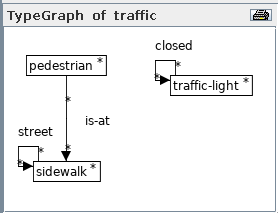
\includegraphics[scale=0.5]{grammar/traffic/type-graph}}}
    \caption{Type Graph of the Grammar}\label{fig:tests:traffic-type-graph}
  \end{subfigure}
  \begin{subfigure}[t]{.5\textwidth}
    \centerline{\fbox{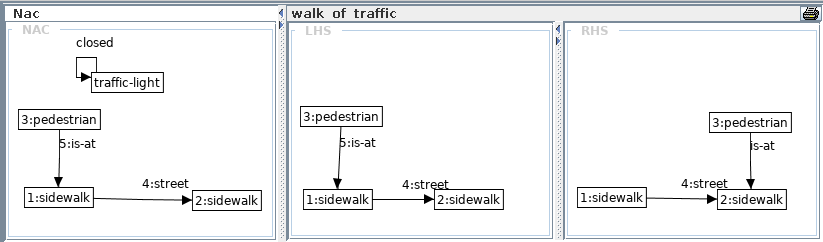
\includegraphics[scale=0.5]{grammar/traffic/walk}}}
    \caption{Rule \emph{walk}}
  \end{subfigure}
  \begin{subfigure}[t]{.5\textwidth}
    \centerline{\fbox{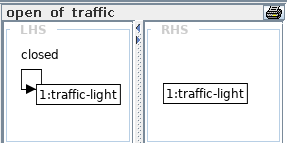
\includegraphics[scale=0.5]{grammar/traffic/open}}}
    \caption{Rule \emph{open}}
  \end{subfigure}%
  \begin{subfigure}[t]{.5\textwidth}
    \centerline{\fbox{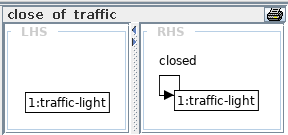
\includegraphics[scale=0.5]{grammar/traffic/close}}}
    \caption{Rule \emph{close}}
  \end{subfigure}
  \caption{Graph Grammar of the Traffic System}\label{fig:tests:grammar-traffic}
\end{figure}

As before, to begin the construction of the occurrence graph grammar with NACs from our graph grammar, we will need a collection of rules and an input-output relation. The chosen collection consists of one copy of each rule in the original grammar. The $IO$ relation is also very simple: it only identifies the traffic lights and the edges that represent they are closed in rules \emph{close} and \emph{open}. The relation is depicted on Figure~\ref{fig:tests:inout-traffic}.

\begin{figure}[!ht]
\centering
\fbox{\includegraphics[scale=0.5]{grammar/traffic/io}}
\caption{Input output relation for the traffic graph grammar}\label{fig:tests:inout-traffic}
\end{figure}

The first step in the construction, the amalgamation of rules, results in the core graph depicted in Figure~\ref{fig:tests:amalgamation-traffic}. Notice that, differently from the type graph in Figure~\ref{fig:tests:traffic-type-graph}, it has concrete elements, a generic pedestrian is now \emph{Jane}, there are two specific sidewalks which are connected by the \emph{Avenue B}, etc.

\begin{figure}[!ht]
  \centering
  \fbox{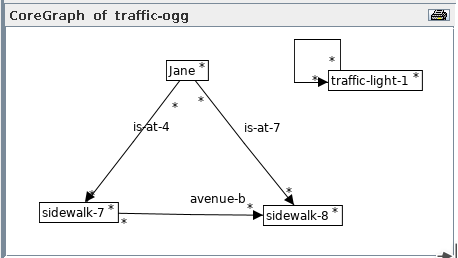
\includegraphics[scale=0.5]{grammar/traffic/amalgamation}}
  \caption{Amalgamation (colimit) of rules for the traffic grammar example.}\label{fig:tests:amalgamation-traffic}
\end{figure}

The second step retypes the rules providing the actions depicted in Figure~\ref{fig:tests:actions-traffic}. Once again, NACs are not shown due to limitations with AGG format compatibility for double-typed graph grammars.

The third step is to calculate the causal relation. For this particular execution of the grammar it consists of the set cointaining only the pair \emph{close} $<$ \emph{open}. Therefore, in this context, the traffic light must be closed before it opens and, so far, the action \emph{walk} does not relate to any of the others. This relation is a partial order, given that there are multiple options of total orderings which respect this relation: $[walk < close < open]$, $[close < walk < open]$ and $[close < open < walk]$.

\begin{figure}[!ht]
  \centering
  \begin{subfigure}[t]{.5\textwidth}
    \centerline{\fbox{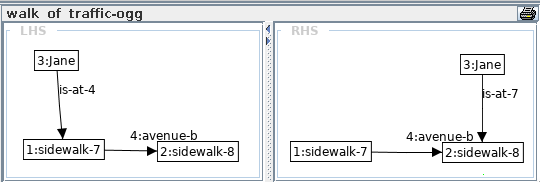
\includegraphics[scale=0.5]{grammar/traffic/amalgamation/walk}}}
    \caption{Action \emph{walk}}
  \end{subfigure}
  \begin{subfigure}[t]{.5\textwidth}
    \centerline{\fbox{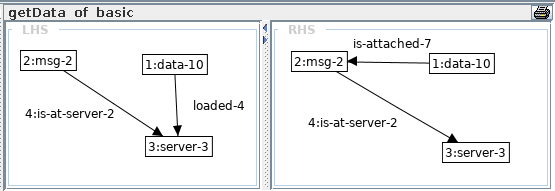
\includegraphics[scale=0.5]{grammar/server/amalgamation/getData}}}
    \caption{Action \emph{open}}
  \end{subfigure}
  \begin{subfigure}[t]{.5\textwidth}
    \centerline{\fbox{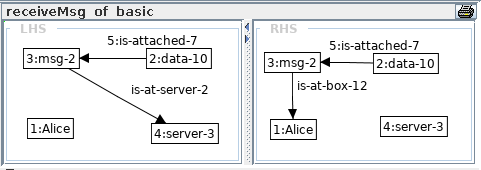
\includegraphics[scale=0.5]{grammar/server/amalgamation/receiveMsg}}}
    \caption{Action \emph{close}}
  \end{subfigure}
  \caption{The set of actions generated for the traffic graph grammar.}\label{fig:tests:actions-traffic}
\end{figure}

After calcultating the causal relation, we construct the \emph{Initial} and \emph{Final} graphs obtained by deletion of elements created (resp. deleted) by the actions in the core graph. The graphs for this execution are shown in Figure~\ref{fig:tests:graphs-traffic}.

\begin{figure}[!ht]
  \centering
  \begin{subfigure}[t]{.5\textwidth}
    \centerline{\fbox{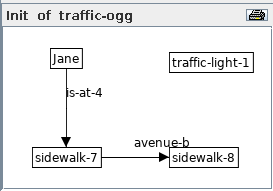
\includegraphics[scale=0.5]{grammar/traffic/init}}}
    \caption{Initial graph}
  \end{subfigure}%
  \begin{subfigure}[t]{.5\textwidth}
    \centerline{\fbox{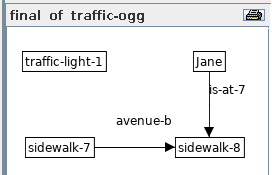
\includegraphics[scale=0.5]{grammar/traffic/final}}}
    \caption{Final graph}
  \end{subfigure}
  \caption{Instance graphs for the traffic grammar}\label{fig:tests:graphs-traffic}
\end{figure}

  The characterization of conflicts and dependencies is where the behaviour of this graph grammar greatly defers from our previous example.
  There is one potential produce-forbid conflict between actions \emph{close} and \emph{walk} and one potential delete-forbid dependency between actions \emph{open} and \emph{walk}.
  Both the conflict and the dependency act over the same triggering element, the \emph{closed} edge in the NAC of action \emph{walk}.
  This element is not present in the \emph{Initial} graph, as it is created by the action \emph{close}.
  Also, the element is not (causally) related to the action \emph{walk}, given that the actions which create and delete it are themselves not related to that action.
  It is easy to see that the action \emph{walk} can either occur before action \emph{close} or after action \emph{open}, but never in between them, because \emph{Jane} must not cross \emph{Avenue B} while the traffic light is closed.
  Therefore, we have an abstract produce-forbid conflict as well as an abstract delete-forbid dependency which, in this case, are both denoted by the tuple $(walk,close, open)$. Moreover, as there are no concrete conflicts and dependencies induced by NACs, the occurrence relation remains equal to the causal relation.

Finally, we have to find at least one total ordering of the actions respecting both the occurrence relation $\leq_o$ = $[close <_o open]$ and the set of occurrence relation restrictions $R = (walk,close,open)$. In fact, there are two such orderings: $[walk < close < open]$ and $[close < open < walk]$. Therefore, the strongly safe graph grammar constructed from this graph grammar execution is also an occurrence graph grammar with NACs.

\section{Generating Tests}

%Once the previous verifications were executed, we can build the occurrence relation to verify whether $OGG_i$ can be really an occurrence graph grammar. If no abstract dependencies or conflicts are found, then the concrete relations are sufficient to perform this verification, and it suffices to check if there is a total ordering compatible with the occurrence relation. If the set $R$ of \emph{occurrence relation restrictions} is not empty, we also need to check if there is a total ordering of the occurrence relation that respects these restrictions.

%As to check wether a partial order satisfies the generated set of restrictions seems to be a hard problem, in the complexity sense, we left this last implementation as a future work.

  Occurrence Graph Grammars may be used to generate a set of tests for a Graph Grammar. The process of constructing an occurrence graph grammar may provide insights for tests even when it fails. In the case where OGGs are found, we have test cases for successful executions of the system under modelling and conditions over how the system should execute. In the case where OGGs are not found, we have test cases for executions where the system must always fail.

We use the occurrence relation and the set of abstract restrictions as test oracles, to define the acceptance of the tests: any path that complies to the format imposed by them is considered valid and must always succeed. On the other hand, paths that break at least one of such restrictions are considered invalid, and their tests must always capture them as failures.

  The tests are represented by the concrete orderings of the rules execution, orderings of elements creation/deletion, and by the initial and final graphs.
  An ordering of rules is one of (possibly) many valid orders in which the rules can be applied according to the occurrence relation. An ordering of elements represents an ordering in which the state of the system may be constructed. While the initial and final graphs translate the valid/necessary data for the input and output of each test. More specific usability details can be found on the Verigraph tutorial, which can be found at \url{https://github.com/Verites/verigraph-tutorial/releases}.


The output of Verigraph for an OGG creation and its test case generation is shown on Figure~\ref{fig:tests:checklist}. On the first figure, Verigraph performs the basic verifications to check whether the generated output is, in fact, an occurrence grammar.

\begin{figure}[!ht]
\caption{Tool command line output}
\begin{minted}[linenos=true, breaklines,fontsize=\small]{shell}
Testing Serialization:
[OK] Unique creations and deletions
[OK] Initial graph is valid
[OK] Final graph is valid
[OK] Concrete occurrence relation is a total order
[OK] Concrete elements relation is a total order
[WARN] There are abstract restrictions
Analysis written in ogg_execution_analysis
Test cases written in ogg_execution_test_cases
Doubly-typed grammar saved in ogg_execution.ggx
\end{minted}
  \label{fig:tests:checklist}
\end{figure}

The analysis file contains a summary of the results for calculation of conflicts and dependencies among rules and among elements. For example: which conflicts and dependencies were found; for the conflicts and dependencies induced by NACs which are the triggering elements of each NAC; the causal relation between elements and actions that created/deleted them, etc. Figure~\ref{fig:tests:analysis} depicts the content of the analysis file for our traffic example.

\begin{figure}[!ht]
\caption{Analysis file content}
\begin{minted}[linenos=true, breaklines,fontsize=\small]{shell}
Conflicts and Dependencies:
[
  Interaction {firstRule = "close", secondRule = "walk", interactionType = ProduceForbid, nacInvolved = Just 0},
  Interaction {firstRule = "close", secondRule = "open", interactionType = ProduceUse, nacInvolved = Nothing},
  Interaction {firstRule = "open", secondRule = "walk", interactionType = DeleteForbid, nacInvolved = Just 0}
]

Creation and Deletion Relation:
[
  (Edge 1,Rule "open"),(Edge 4,Rule "walk"),(Rule "close",Edge 1),(Rule "walk",Edge 7)
]

Conflicts and dependencies induced by NACs:
[
  (Interaction {firstRule = "close", secondRule = "walk", interactionType = ProduceForbid, nacInvolved = Just 0},Edge 1),
  (Interaction {firstRule = "open", secondRule = "walk", interactionType = DeleteForbid, nacInvolved = Just 0},Edge 1)
]
\end{minted}
  \label{fig:tests:analysis}
\end{figure}


The test cases file contains information we consider relevant to a test designer, such as the rules and elements involved in that particular execution of the graph grammar represented by the occurrence graph grammar, as well as the occurrence relation, a total ordering of rules application (if found) and the set of restrictions (if found). Figure~\ref{fig:tests:cases} presents the content of the test cases files for our traffic example.


\begin{figure}[!ht]
\caption{Test cases file content}
\begin{minted}[linenos=true, breaklines,fontsize=\small]{shell}
Rules involved:
[Rule "close",Rule "open",Rule "walk"]

Concrete Rules Relation:
[(Rule "close" < Rule "open")]

Elements involved:
[Node 1,Node 7,Node 8,Node 9,Edge 1,Edge 3,Edge 4,Edge 7]

Elements Relation:
[(Edge 4 < Edge 7)]

Rules Ordering: Just [Rule "close",Rule "open",Rule "walk"]

Elements Ordering: Just [Node 1,Node 7,Node 8,Node 9,Edge 1,Edge 3,Edge 4,Edge 7]

Set of Abstract Restrictions:
[
  (AbstractProduceForbid: Rule "walk" must not occur between [Rule "close" < Rule "open"]),
  (AbstractDeleteForbid: Rule "walk" must not occur between [Rule "close" < Rule "open"])
]
\end{minted}
  \label{fig:tests:cases}
\end{figure}

Finally, the \code{.ggx} file presents a translation of the constructed occurrence graph grammar from Verigraph format to AGG format in order to support the OGG graphical visualization. It contains its actions (without NACs), initial and final graphs and core graph (which assumes the role of the type-graph in AGG) as shown in the previous section.

